\chapter{迁移学习和持续学习的可学习性}
\label{chap:transfer-learning-theory}

一个邮件分类器可以在过去月份的样本上达到很低的错误率，但这份结果还不能回答三个后续问题。新月份的邮件分布改变后，它能否继续识别诈骗邮件？邮件来源不变而误判代价改变后，已有模型能否支持新的决策？如果邮件不断到来、旧数据逐渐无法重访，模型能否一边适应新邮件，一边保持对历史邮件的识别能力？三个问题都要求把有限经验得到的结果用于总体，但可用信息和评价目标各不相同。

前几章已经建立总体风险、超额风险和PAC可学习性的分析方法。本章沿用这些对象，分别考察分布变化下的迁移、任务变化下的迁移，以及固定任务下的持续学习。我们先判断可见信息是否足以支持所需预测，再构造能够估计目标风险的学习过程，最后检查样本量、优化误差和记忆限制。反例用于说明哪些信息缺口不能靠增加同类样本弥补；正面结论则明确算法在什么范围内能够学会。

以下有限样本结论中，样本数与有限候选数均为正整数，失败概率$\delta\in(0,1)$，优化误差非负；需要条件分布时，假定相应条件概率核存在。

\section{迁移学习和持续学习的设定与挑战}
\label{sec:transfer-learning-setting}

在此前常用的设定中，我们先固定任务、损失和假设空间，再从同一未知分布独立抽取训练样本，并评价算法在这个分布上的总体风险。经验风险与总体风险由同一个分布联系起来，有限样本分析控制二者的偏差。本章改变其中的分布、任务或数据访问方式；这些改变决定了原有证明中哪一步还可沿用，哪一步需要新的条件。

\Needspace{7\baselineskip}
\subsection{迁移学习的设定}
\label{sec:transfer-settings-overview}

\subsubsection{任务不变时的分布变化}

邮件分类的输出仍是“正常”或“诈骗”，两类错误的计分方式也保持不变，但邮件长度、类别比例或给定特征后的诈骗概率可能变化。把输入与标签记为$(x,y)$，源域和目标域分别由联合分布$\mathcal P_S,\mathcal P_T$描述。任务固定意味着我们在两个分布上使用同一种损失；它不要求两个分布拥有相同的最优分类器。

算法能看到哪些目标信息，需要单独约定。\term{领域自适应}（domain adaptation）允许目标域数据参与学习；无监督领域自适应只提供目标输入，不提供目标标签。\term{领域泛化}（domain generalization）则在训练和模型选择时都不使用目标数据，要求训练所得模型直接用于允许的新环境。部署时读取一个待预测输入，与用一批目标数据更新模型，是不同的信息访问方式。

\subsubsection{数据分布不变时的任务变化}

同一批邮件也可以服务不同的决策要求。例如，原先把漏判诈骗与误拦正常邮件计为相同代价，后来要求尽量减少误拦；数据的特征、标签及其联合分布没有变化，最优决策却可能改变。我们用固定分布$\mathcal P$和两个损失$\ell_S,\ell_T$表达这一情形。任务变化改变的是评价同一预测的方式，迁移需要判断旧任务留下的信息能否支持新目标。

可复用的知识可能是一个分类器，也可能是预测概率、特征表示或统计摘要。它们保留的信息不同，不能只因都称为“已有模型”就赋予相同的理论保证。如果任务改变了预测标签，例如从识别诈骗转为识别邮件主题，应先固定底层邮件来源，再分别说明标签如何产生；此时新的特征--标签联合分布并没有自动保持不变。本章先在固定观测分布、改变损失的设定中给出可核查的结论。

\Needspace{7\baselineskip}
\subsection{持续学习的设定}
\label{sec:continual-settings-overview}

\subsubsection{持续到达的数据与分布变化}

现在让邮件按月份到达，模型每接收一批数据便更新，并继续承担分类任务。本章主要固定输入输出的含义和损失，允许第$t$个阶段的分布$\mathcal P_t$随时间改变；分布始终相同也是其中一种情形。阶段可以是明确的数据批次，理论分析中的阶段划分不意味着现实系统总能准确检测到变化边界。

每次更新都可能包含一次从历史分布到当前分布的迁移。但持续学习还要评价更新后的模型在历史分布上是否仍能完成任务。因而，连续适应当前数据只是过程的一部分，整个序列上的评价要求也必须进入学习问题。

\subsubsection{历史数据访问与知识保留}

如果全部历史邮件都能反复读取，我们可以在每次更新时重新汇集数据。持续学习中的资源限制使这种做法未必可用：旧数据离开后，算法只能利用保留下来的状态。这个状态可以包含模型参数、少量样本和统计摘要，其容量与更新方式都应列为条件。

“没有保存旧样本”并不意味着没有保存历史信息。例如，对每个有限候选模型累计过去的损失，就能保留某些学习目标所需的统计量。反过来，若允许用无限精度实数存放全部过去，也不能把这种形式上的固定维状态解释为有限记忆。后面的存储分析会明确计数精度或可用比特数。

\subsubsection{当前适应与历史表现保持}

更新后的模型既要在当前月份的总体上表现良好，也可能需要处理再次出现的历史邮件类型。我们把吸收新数据、改善当前预测的要求称为可塑性，把保持仍有用的历史能力的要求称为稳定性。这里的稳定性评价能力随更新如何变化，与替换训练样本所定义的算法稳定性具有不同含义。

历史表现还可以有不同的评价口径。历史分布上的平均错误率允许少数月份表现较差；要求每个历史分布的错误率都小则更强。如果相同输入在不同月份必须得到相反标签，而预测时又不提供月份信息，同一个分类器可能无法同时达到各月份自己的最优风险。因此，保持要求必须连同允许的分布序列和比较基准一起规定。

\Needspace{7\baselineskip}
\subsection{与一般可学习性问题的区别和挑战}
\label{sec:transfer-continual-challenges}

\subsubsection{训练样本与评价总体之间的联系}

源域训练误差首先估计源域风险。即使这个估计完全准确，我们仍需说明它为什么能限制目标域风险。源域是否覆盖目标输入、标签规律之间存在什么联系、目标标签是否可用，都会影响这一转换。缺少必要联系时，可见数据可能完全相同而正确的目标决策不同，困难便发生在抽样误差之前。

跨分布结论也需要说明针对哪个总体作出承诺。对每个预先允许的目标域分别保证，与对随机抽取的新环境平均保证，约束的是不同对象。前者不能仅由后者推出；增加某个已有环境内的样本，也不能普遍替代增加独立环境的数量。

\subsubsection{已有知识对新学习目标的适用性}

任务改变以后，源任务上的最优结果可能没有保留目标任务所需的全部信息。例如，一个只输出类别的模型没有直接报告类别概率，而新的误判代价可能要求按概率重新选择阈值。因此，源任务完成得好与目标任务能够从旧知识中学会，是两个需要分别证明的判断。

如果原始数据仍完整可用，而且新损失能由这些数据计算，按新目标重新学习就是一个基准。迁移的额外价值应体现为目标任务需要更少的新样本或计算。这样的收益依赖任务联系；只证明目标任务可学习，还不能证明旧知识带来了收益。

\subsubsection{有限历史信息下的稳定性与可塑性}

持续学习把风险控制扩展到多个更新阶段。当前训练样本可以帮助估计当前风险，却不能直接检验已经不可访问的所有历史分布。算法必须通过保留信息、共享预测规律或其他明确条件，把历史保证传递到下一阶段。

单次更新有保证，也不意味着整个过程自动具有相同保证。更新次数增加可能累积风险增量和失败概率，历史平均风险还可能掩盖个别环境的遗忘。我们需要同时说明样本量、记忆容量、序列长度与评价精度的关系。表达能力限定可以达到的风险，优化误差说明算法离经验目标还有多远，泛化分析则把经验结果连接到所评价的总体。

\section{分布变化下的迁移可学习性}
\label{sec:domain-adaptation}

先回到任务固定、月份改变的邮件分类问题。要从旧邮件学习新月份的分类器，我们需要依次确定三件事：算法能使用什么信息，源标签如何与目标标签联系，以及有限样本是否足以估计这种联系所定义的风险。本节以无监督领域自适应为主要设定，并在目标数据完全不可用时讨论领域泛化。

\Needspace{7\baselineskip}
\subsection{学习问题}
\label{sec:adaptation-generalization-settings}

\subsubsection{固定任务与变化的联合分布}
\label{sec:distribution-shift}

固定可测输入空间$X$、标签空间$Y$和取值于$[0,1]$的损失$\ell$。联合分布既可分解为输入分布与条件标签分布，也可分解为类别比例与类内输入分布：
\[
 \mathcal P(x,y)=\mathcal P^X(x)\mathcal P(y\mid x)
               =\mathcal P^Y(y)\mathcal P(x\mid y).
\]
这里的乘积表示相应边缘分布与条件概率核的组合；离散情形可直接按概率相乘。比较这些组成部分，可以说明迁移保留了什么关系，而不仅是说“数据变了”。

协变量偏移（covariate shift）保留$\mathcal P(y\mid x)$，允许$\mathcal P^X$变化；相同邮件特征对应的标签概率不变，但不同特征出现的比例改变。标签偏移（label shift）保留$\mathcal P(x\mid y)$，允许类别比例变化；它通常也会改变由输入反推标签的概率。\term{概念偏移}（concept shift）直接描述$\mathcal P(y\mid x)$变化。这些条件可以交叉，不能理解为互斥分类；图~\ref{fig:learning-distribution-shift}展示了被改变的分布成分。

\begin{figure*}[htbp]
  \centering
  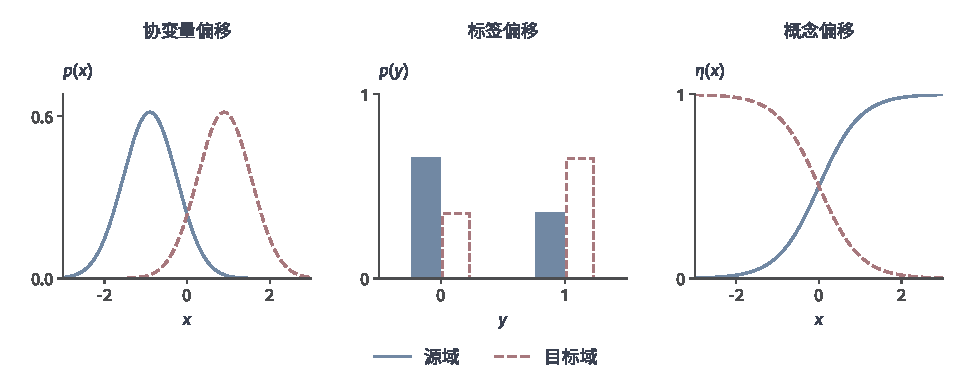
\includegraphics[width=164.600mm]{figures/03-foundations/02-learning-theory/matplotlib/learning-theory-distribution-shift/figure.pdf}
  \caption{分布偏移改变联合分布的不同组成部分。实线表示源域，虚线表示目标域；密度、类别比例和条件概率均为规范化的教学构造，不表示实测频率。协变量偏移允许输入分布改变，标签偏移允许类别比例改变，概念偏移则改变给定输入后的标签分布，图中$\eta(x)=\mathbb P(y=1\mid x)$。这些设定还需与覆盖条件或其他可识别条件结合，才能支持迁移保证。}
 \label{fig:learning-distribution-shift}
\end{figure*}
\FloatBarrier

\subsubsection{源域数据、目标域信息与评价目标}
\label{sec:transfer-pac-setting}

为了区分“在哪个总体上表现好”，对同一假设$h\in\mathcal H$定义
\begin{equation}
 R_D(h)=\mathbb E_{(x,y)\sim\mathcal P_D}\ell(h(x),y),
 \qquad D\in\{S,T\}.
 \label{eq:transfer-population-risks}
\end{equation}
目标域可能有标签噪声，假设空间也可能存在表达限制。因此，我们用$R_{T,\mathcal H}^{\star}=\inf_{h\in\mathcal H}R_T(h)$作为比较基准，称$R_T(h)-R_{T,\mathcal H}^{\star}$为\term{目标域超额期望风险}（target-domain excess risk）。它衡量所选假设与同一候选空间中目标表现最优者的差距。

无监督领域自适应接收相互独立的带标签源样本$S_S\sim\mathcal P_S^{n_S}$与无标签目标样本$U_T\sim(\mathcal P_T^X)^{n_T}$。能否学习取决于允许的分布对集合$\mathfrak P_{\mathrm{DA}}$；覆盖关系、共享标签规律、已知辅助信息都属于这个设定。以下概率包含抽样与算法内部随机性，并假定涉及的损失、上确界和输出满足可测性要求。

\begin{definition}[领域自适应的PAC可学习性]
\label{def:adaptation-pac-learnability}
固定$\mathcal H,\ell,\mathfrak P_{\mathrm{DA}}$。若存在输出属于$\mathcal H$的算法$A$和有限门槛$m_S,m_T$，使对任意$\varepsilon,\delta\in(0,1)$、任意$(\mathcal P_S,\mathcal P_T)\in\mathfrak P_{\mathrm{DA}}$，以及$n_S\geq m_S(\varepsilon,\delta)$、$n_T\geq m_T(\varepsilon,\delta)$，都有
\[
 \mathbb P\{R_T(A(S_S,U_T))-R_{T,\mathcal H}^{\star}\leq\varepsilon\}
 \geq1-\delta,
\]
则称该设定PAC可学习。门槛可以依赖假设空间和分布族的统一参数，但不能依赖未知的具体分布对。
\end{definition}

这个要求约束总体风险，并不是说源域上观察到的任意规律都会在目标域成立。若需要已知密度比等辅助输入，必须把它写进算法的信息条件。定义先要求有限样本下存在成功算法；高效计算还需要另外控制求解代价。

\Needspace{7\baselineskip}
\subsection{可学习的条件}
\label{sec:adaptation-risk}

\subsubsection{目标预测规律的可识别性}

设两个月份都以相同概率产生输入0和1，源标签为$y=x$，目标标签却可能是$y=x$或$y=1-x$。源标签样本与无标签目标输入在两种情形中的分布完全一样，正确决策却相反。图~\ref{fig:learning-alignment-counterexample}把同一预测与两种隐藏标签并排比较，说明输入分布对齐仍不足以确定目标预测。

\begin{figure*}[!htb]
  \centering
  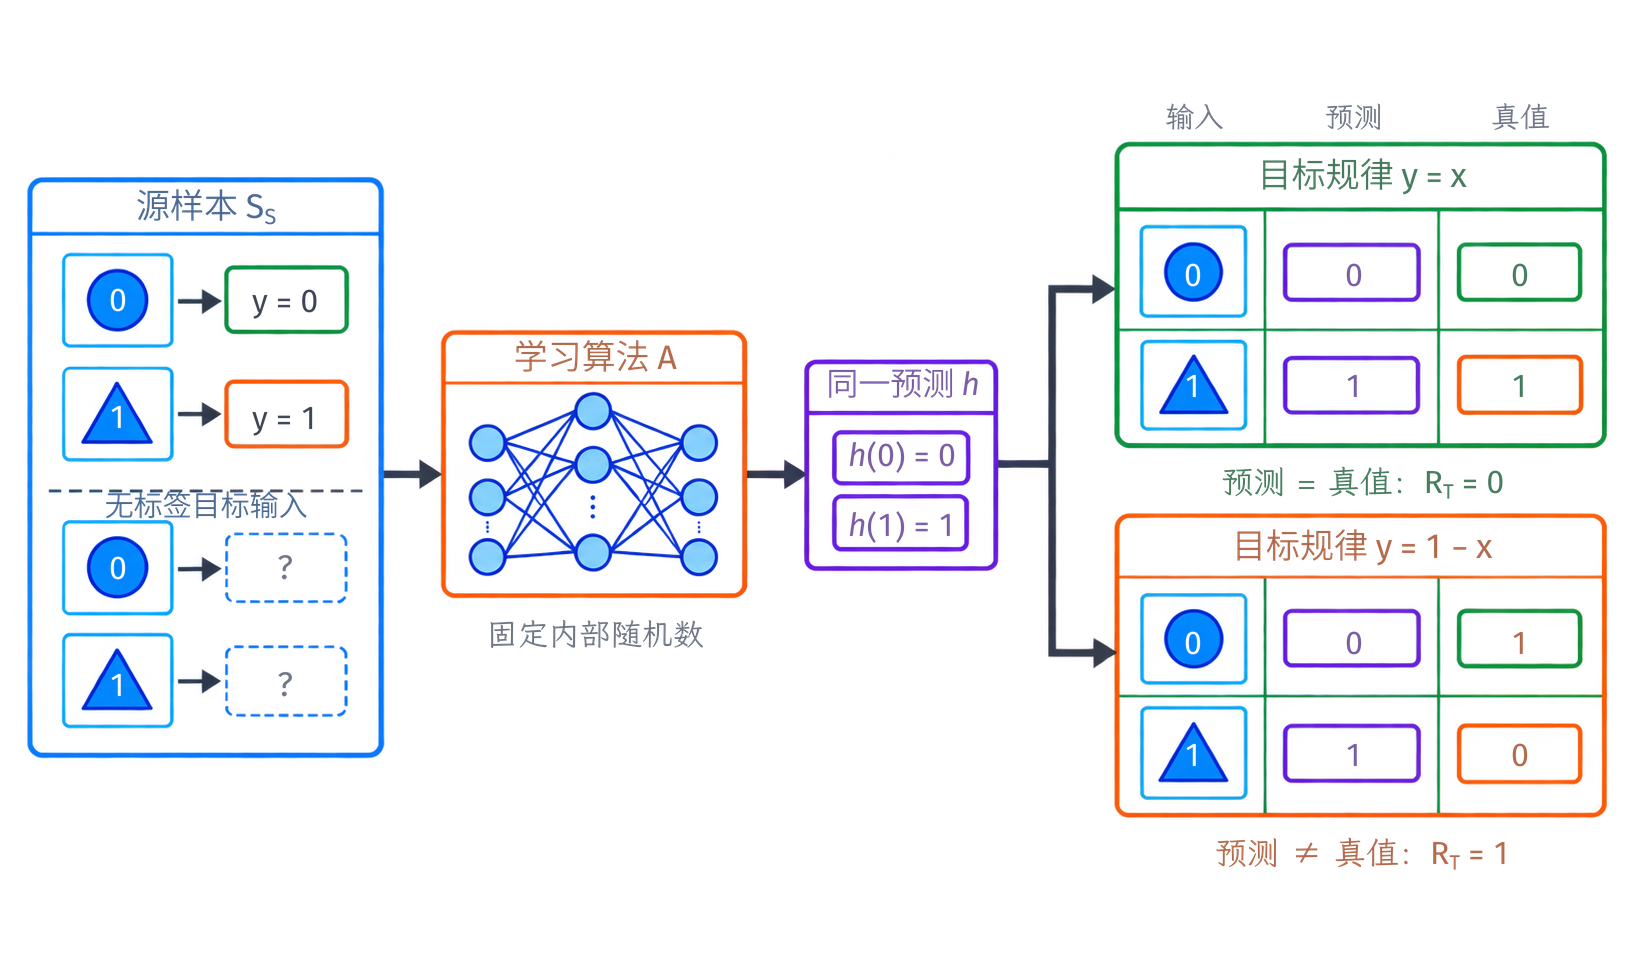
\includegraphics[width=164.600mm]{figures/03-foundations/02-learning-theory/generated/learning-theory-alignment-counterexample/figure.png}
  \caption{相同可观察数据不能区分两种目标规律。两域都以概率$1/2$产生输入0或1，源标签为$y=x$。算法只收到左侧带标签源样本和无标签目标域训练样本，目标标签并未提供；右侧两种可能分别取$y=x$与$y=1-x$。固定算法内部随机数后，两种情形必得到同一训练分类器。图中以$h(x)=x$为例，两张表逐点对照同一预测与隐藏标签：零一损失下，源风险为0，两种目标风险分别为0、1。任意二分类器在这两种目标规律下的风险之和为1。输入完全对齐仍未提供选择目标规律的证据，还需目标标签或连接两域标签规律的额外条件。}
  \label{fig:learning-alignment-counterexample}
\end{figure*}
\FloatBarrier

一个目标量是否由可观察数据的分布唯一确定，是\term{可识别性}（identifiability）问题。预测学习还需核对识别的对象：不同的条件标签概率可能拥有相同的最优决策，例如正类概率为0.7或0.8时都应预测1。用这一思路证明不可学习，需要可见规律相同而近似最优决策不能兼容的反例，不能只指出标签概率不同（可参考\BookChapterRef{chap:random-variables}{卷2“随机变量”章}）。

\subsubsection{分布覆盖与跨域风险的联系}

源域从未出现的目标输入，需要额外的标签联系才能预测。若目标输入分布对源输入分布绝对连续，即$\mathcal P_T^X\ll\mathcal P_S^X$，源域零概率集合在目标域也为零概率。图~\ref{fig:learning-support-coverage}显示覆盖与密度相同是两种要求：源、目标密度可以不同，但缺少覆盖的区域无法仅靠更多源观测补出标签。

\begin{figure*}[!htb]
  \centering
  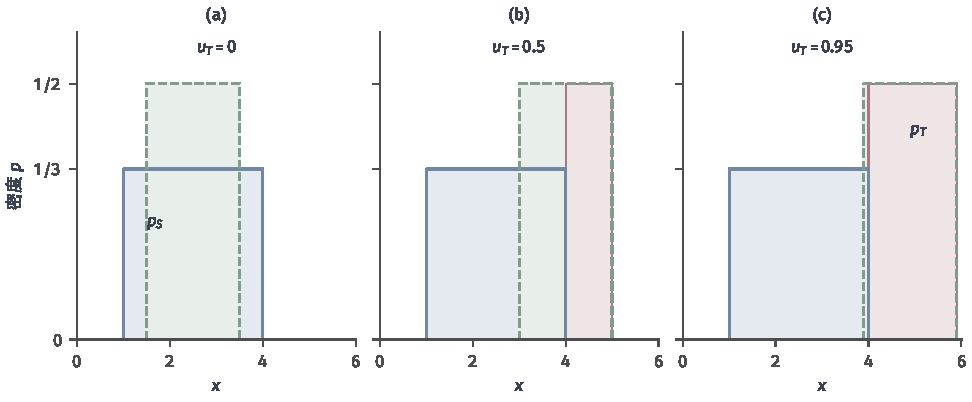
\includegraphics[width=164.600mm]{figures/03-foundations/02-learning-theory/matplotlib/learning-theory-support-coverage/figure.pdf}
  \caption{同尺度的三种支持覆盖。源密度均为$[1,4]$上的$1/3$，目标密度均为长度2区间上的$1/2$；(a)、(b)、(c)的目标支持依次为$[1.5,3.5]$、$[3,5]$、$[3.9,5.9]$。深色区域没有源密度，其目标概率$u_T=\mathbb P_T\{p_S(X)=0\}$依次为0、0.5、0.95。实线、虚线与底色共同区分源域、目标域；只有(a)满足覆盖条件$p_T(x)>0\Rightarrow p_S(x)>0$。密度为规范化教学构造，不是实验分布。}
 \label{fig:learning-support-coverage}
\end{figure*}
\FloatBarrier

另一种连接两域风险的办法，是比较分类器之间的预测分歧。分歧只涉及输入，因此可以在无标签目标样本上观察。对二分类零一损失，令
\begin{equation}
 d_{\mathcal H\triangle\mathcal H}
 =2\sup_{h,g\in\mathcal H}
 \left|\mathbb P_S^X(h\neq g)-\mathbb P_T^X(h\neq g)\right|,
 \label{eq:h-delta-h-divergence}
\end{equation}
其中$h\neq g$表示二者在同一输入上给出不同类别。上确界覆盖算法可能选出的全部假设对，系数2采用假设分歧散度的惯用归一化。还需定义$\lambda=\inf_{g\in\mathcal H}(R_S(g)+R_T(g))$，衡量同一个候选在两域上能达到多小的风险之和。

\begin{theorem}[领域自适应的目标域期望风险界]
\label{thm:domain-adaptation-bound}
对非空可测二分类假设空间$\mathcal H$和源、目标联合分布，采用零一损失及上述分歧散度与$\lambda$，则每个$h\in\mathcal H$都满足
\begin{equation}
 R_T(h)\leq R_S(h)+\tfrac12d_{\mathcal H\triangle\mathcal H}+\lambda.
 \label{eq:domain-adaptation-risk-bound}
\end{equation}
\end{theorem}
\begin{proof}
固定任意$g\in\mathcal H$。若$h$在目标域出错，则$g$出错或二者预测不同，故
$R_T(h)\leq R_T(g)+\mathbb P_T^X(h\neq g)$。散度定义把后一项限制为
$\mathbb P_S^X(h\neq g)+d_{\mathcal H\triangle\mathcal H}/2$。
在源域，预测不同意味着至少一者出错，因此
$\mathbb P_S^X(h\neq g)\leq R_S(h)+R_S(g)$。合并并对$g$取下确界即可。
\end{proof}

该界分别保留源风险、输入差异和标签相关量\scite{bendavid2010adaptation}。其中$\lambda$包含目标标签，不能从无标签输入直接估计；它也可能因两域共有噪声而为正，不能据此断言目标超额风险不可学习。图~\ref{fig:learning-domain-classifier}用域分类错误解释输入散度：域先验相等、判别类对取补封闭时，其最小错误$e^*$与相应散度满足$d=2(1-2e^*)$。能分清输入来源，只说明输入差异，不决定目标任务的全部风险。

\begin{figure*}[!htb]
  \centering
  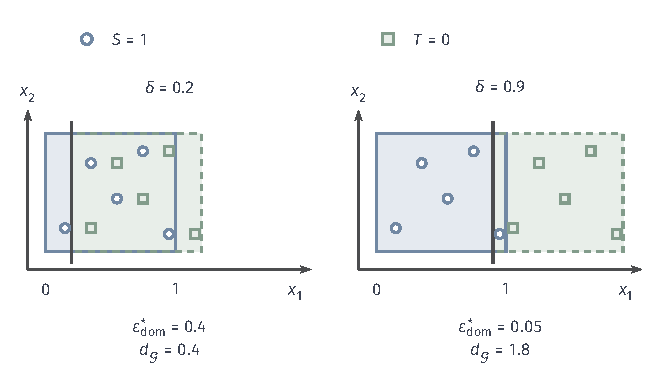
\includegraphics[width=113.404mm]{figures/03-foundations/02-learning-theory/tikz/learning-theory-domain-classifier/figure.pdf}
  \caption{域分类器的错误只对应输入散度项。源输入均匀分布于$[0,1]^2$，目标输入均匀分布于$[\delta,1+\delta]\times[0,1]$，其中$0\leq\delta\leq1$；圆点、方块的位置为教学构造，错误率由区域概率计算。$\mathcal H$含双向阈值与常值假设，域分类器类取$\mathcal G=\mathcal H\triangle\mathcal H$。其中$g=h_0\mathbin\oplus h_\delta$在左侧浅色带预测源域，$h_a(x)=\mathbb I\{x_1\geq a\}$；两域均等先验时，最小域错误为$(1-\delta)/2$，$d_{\mathcal G}=2\delta$。任务风险界还包含源风险及$\lambda=\inf_{h\in\mathcal H}(R_S(h)+R_T(h))$，不能只由域错误决定。}
 \label{fig:learning-domain-classifier}
\end{figure*}
\FloatBarrier

\subsubsection{缺少跨域联系时的不可学习性}

现在把信息缺口写成一个有限样本也无法消除的结论。下面只有两个候选分类器，每种可能的目标机制都能被其中一个正确表示；失败来自可见信息无法在二者之间作出选择。

\begin{theorem}[缺少覆盖时的不可学习性]
\label{thm:transfer-nonidentifiability}
采用二分类零一损失。令$X=\{a,b\}$、$Y=\{0,1\}$，且
$\mathcal H=\{h_0,h_1\}$满足
\[
 h_0(a)=h_1(a)=0,\qquad h_0(b)=0,\quad h_1(b)=1.
\]
源域分布$\mathcal P_S$恒产生$(a,0)$，目标域输入边缘分布恒产生$b$。
允许的两个目标域分布$\mathcal P_T$分别令$b$的标签恒为0或恒为1，并定义
$R_T(h)=\mathbb P_{(x,y)\sim\mathcal P_T}\{h(x)\neq y\}$。
对任意$n_S,n_T\geq1$，令
$S_S\sim\mathcal P_S^{n_S}$、
$U_T\sim(\mathcal P_T^X)^{n_T}$相互独立。
对任意只使用带标签源域样本与无标签目标域样本、输出属于$\mathcal H$的可能随机化
学习算法$A$，无论两类样本量多大，总有一个允许的目标域满足
\[
 \mathbb P_{S_S,U_T,A}\!\left(
 R_T(A(S_S,U_T))>\tfrac14
 \right)\geq\tfrac12.
\]
这里概率包含抽样与算法内部的随机性。两个设定各自都存在源域与目标域期望风险同时为零的假设。
\end{theorem}
\begin{proof}
两种设定中，算法收到的全部源域样本都是$(a,0)$，全部目标域输入都是$b$，因此
输入数据的分布完全相同。设算法输出$h_1$的概率为$p$；这个概率只可能来自算法内部
随机性，且在两个设定中相同。目标标签为0时，算法以概率$p$输出$h_1$，其目标域
零一风险为1；目标标签为1时，算法以概率$1-p$输出$h_0$，其目标域零一风险也为1。
两者至少有一个不小于$1/2$。标签为0的设定中$h_0$在两域均无错误，标签为1的设定中
$h_1$在两域均无错误，故失败并非假设空间缺少合适的假设。
\end{proof}

无论样本量多大，输入$b$的标签都没有进入观测。这里甚至存在同时在源域和目标域零风险的候选，所以“存在一个好模型”也不能代替识别该模型的依据。不可学习结论依赖这一允许分布族；提供目标标签或增加有效的跨域联系会改变问题\scite{bendavid2010impossibility}。

\Needspace{7\baselineskip}
\subsection{有限样本保证}

\subsubsection{重加权学习的目标域风险保证}
\label{sec:adaptation-coverage}

若两个域共享条件标签核$\mathsf K(\mathrm dy\mid x)$，并且源输入覆盖目标输入，就可以调整源样本的贡献来计算目标风险。令密度比$w=\mathrm d\mathcal P_T^X/\mathrm d\mathcal P_S^X$，其含义是把源输入概率转换为目标输入概率所需的权重。结合共享标签核，得到
\begin{equation}
 R_T(h)=\mathbb E_{(x,y)\sim\mathcal P_S}[w(x)\ell(h(x),y)].
 \label{eq:covariate-risk-identity}
\end{equation}
权重只改变输入的抽样比例，源标签能够用于目标评价仍依赖共享条件核。图~\ref{fig:learning-importance-weighting}展示目标更常见的输入如何获得更大的源样本权重。

\begin{figure}[htbp]
  \centering
  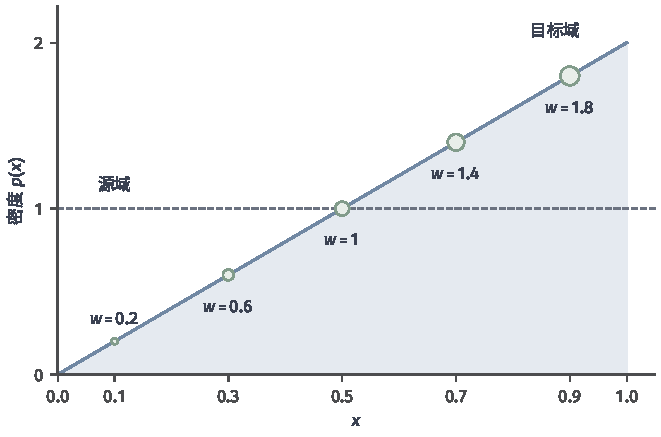
\includegraphics[width=112.000mm]{figures/03-foundations/02-learning-theory/matplotlib/learning-theory-importance-weighting/figure.pdf}
  \caption{重要性权重重新分配源样本的贡献。在$[0,1]$上构造源密度$p_S(x)=1$、
 目标密度$p_T(x)=2x$，二者均积分为1，因此$w(x)=2x$。
 五个源样本位置人为取为0.1、0.3、0.5、0.7、0.9，权重依次为0.2、0.6、1、1.4、1.8。
 圆点叠在目标密度上，面积与权重成正比，面积不表示局部样本数量。
 目标输入必须受到源输入覆盖；要使用风险恒等式，还需保持相同的条件标签分布。}
 \label{fig:learning-importance-weighting}
\end{figure}
\FloatBarrier

为了控制有限样本的波动，还需限制权重大小。设$0\leq w\leq\kappa$，$w$已知，$\mathcal H$包含$N$个可测候选。对$n$个独立源样本计算
$\widehat R_w(h)=n^{-1}\sum_{i=1}^n w(x_i)\ell(h(x_i),y_i)$，并选取其近似最小者。下面允许非零优化误差，明确把统计保证与求解要求接在一起。

\begin{theorem}[已知密度比下的迁移样本量界]
\label{thm:covariate-finite-pac}
在上述共享标签核、覆盖、已知有界密度比及有限假设空间条件下，若算法输出满足
$\widehat R_w(\widehat h)\leq\min_{h\in\mathcal H}\widehat R_w(h)+\rho$，其中$\rho\geq0$，则以概率至少$1-\delta$，
\begin{equation}
 R_T(\widehat h)-R_{T,\mathcal H}^{\star}
 \leq\kappa\sqrt{\frac{2\log(2N/\delta)}{n}}+\rho.
 \label{eq:covariate-finite-excess}
\end{equation}
\end{theorem}
\begin{proof}
每个加权损失在$[0,\kappa]$中。Hoeffding不等式及对$N$个候选的概率求和给出同一个事件，在该事件上
\[
 \sup_{h\in\mathcal H}|\widehat R_w(h)-R_T(h)|
 \leq a_n=\kappa\sqrt{\frac{\log(2N/\delta)}{2n}}.
\]
取目标风险最小者$h^\star$，依次用两次偏差界与一次近似经验最优性，得到
\[
 R_T(\widehat h)\leq\widehat R_w(\widehat h)+a_n
 \leq\widehat R_w(h^\star)+\rho+a_n
 \leq R_T(h^\star)+\rho+2a_n.
\]
\end{proof}

当各候选的损失可计算且候选间的比较可实现时，精确枚举可令$\rho=0$，此时$n\geq2\kappa^2\log(2N/\delta)/\varepsilon^2$足以保证超额风险不超过$\varepsilon$。这是相对于统一权重上界的充分样本量，不是最优下界。若枚举候选过于昂贵，还要另行分析具体优化算法；有限样本可学习与计算高效不能互相替代。

\subsubsection{源样本与目标样本的数量要求}

已知$w$的结论没有使用无标签目标样本，因为分布差异已经由辅助输入提供。当$w$未知时，目标样本的作用是帮助估计它。设从独立辅助数据得到$0\leq\widehat w\leq\kappa$，并以概率至少$1-\delta_w$满足
\[
 \mathbb E_{x\sim\mathcal P_S^X}|\widehat w(x)-w(x)|\leq b_w.
\]
由于损失不超过1，把$w$换成$\widehat w$对每个候选的总体加权风险至多造成$b_w$误差。条件于辅助数据，对新的独立源标签样本使用上一证明，目标超额风险至多增加$2b_w$，总失败概率至多为$\delta_w+\delta_\ell$，其中$\delta_\ell$是损失估计的失败概率。

因此，源样本量控制加权损失的估计，目标样本量通过密度比估计影响$b_w$。沿这条路径推出PAC可学习，需要在允许的分布族上使两类误差都能一致减小；仅有有限假设空间，并不保证任意密度比都能可靠估计。若共享标签核仅近似成立，目标输入平均下的条件标签总变差为$b_{\mathrm{cond}}$，同样会给超额风险上界增加$2b_{\mathrm{cond}}$。固定残余项使当前上界不足以证明任意精度，但不等同于不可学习性下界。

标签偏移也需要先建立可估计的联系。若源域各类别均有正概率、类内分布$\mathsf K_y$保持不变，目标输入分布满足$\mathcal P_T^X=\sum_y q_y\mathsf K_y$，其中$q_y$为目标类别比例。只有这组混合比例可以识别并稳定估计，按类别比例重加权才有依据。类内分布相同的两个类别无法仅凭目标输入区分比例；对于有限类别，类内分布线性无关可保证全体比例的唯一性。有限样本下还需控制可辨程度：当两组类别比例的绝对差之和超过给定阈值时，对应输入分布之间的总变差不能任意接近零，否则抽样波动会掩盖需要识别的比例差异。

\subsubsection{复杂度与算法稳定性带来的保证}
\label{sec:transfer-stability}

有限候选方便展示证明的机制，实际模型可能有无限多个参数取值。此时需要控制加权损失函数族的一致估计误差。例如，独立源样本上的经验Rademacher复杂度为
\[
 \widehat{\mathfrak R}_S(w\ell_{\mathcal H})
 =\mathbb E_{\bm\sigma}\sup_{h\in\mathcal H}
 \frac1n\sum_{i=1}^n\sigma_i w(x_i)\ell(h(x_i),y_i),
\]
其中$\sigma_i$独立等概率取$\pm1$。这个量检验候选加权损失对随机符号的拟合能力；它必须作用于实际重加权后的函数族。沿用前文的对称化与有界差分分析，以概率至少$1-\delta$，
\[
 \sup_h|R_T(h)-\widehat R_w(h)|
 \leq2\widehat{\mathfrak R}_S(w\ell_{\mathcal H})
      +3\kappa\sqrt{\frac{\log(4/\delta)}{2n}}.
\]
这里对正、负两个偏差事件合并，假定相应上确界可测。近似ERM的超额风险仍由右侧的两倍加优化误差控制，跨域条件则仍由式~\eqref{eq:covariate-risk-identity}提供。

另一条路径直接控制算法对样本替换的敏感度。设替换一个源样本后，算法输出在任意观测上的期望未加权损失变化至多为$\beta_n$，且其期望加权经验优化误差至多为$\rho_n$。乘上固定权重后，损失敏感度至多为$\kappa\beta_n$。由于目标风险等于加权源风险，前文的算法稳定性分析给出
\begin{equation}
 \mathbb E\big[R_T(A(S))-R_{T,\mathcal H}^{\star}\big]
 \leq\kappa\beta_n+\rho_n.
 \label{eq:transfer-stability-excess}
\end{equation}
其依据是把超额风险分成期望泛化差与经验优化差，再用
$\mathbb E\inf_h\widehat R_w(h)\leq\inf_hR_T(h)$处理比较基准。若右侧在允许族上一致趋零，非负超额风险的Markov不等式便把期望界转为PAC保证。

复杂度与算法稳定性提供不同的有限样本控制方式，但都没有创造跨域标签联系。采用PAC--Bayes分析随机预测器时也一样：源样本选择参数分布的代价可以被控制，目标标签机制仍需单独建立依据。因而，这些工具应接在可识别条件之后使用，不能把一个随样本量减小的估计项当作完整的迁移结论。

\subsubsection{目标数据不可用时的领域泛化保证}
\label{sec:domain-generalization}

如果训练时没有目标输入，也没有其他目标信息，就不能仅凭源数据估计任意未知目标的密度比。正面结论需要限制允许的新环境。这里比较两种不同的承诺：\term{逐目标域领域泛化}（target-wise domain generalization）要求同一学习程序对每个允许目标域分别给出保证；\term{环境平均领域泛化}（environment-average domain generalization）把训练环境与新环境看成同一环境总体的随机抽样，评价新环境上的平均风险。后者允许某些环境风险较高。

先看逐目标域的一个充分条件。对二分类，假定训练与允许的目标域共享条件正类概率$\eta(x)$，且$h^\star(x)=\mathbb I\{\eta(x)\geq1/2\}$属于有限空间$\mathcal H$。令训练混合分布为$\overline{\mathcal P}$，对每个目标都满足$\mathcal P_T^X\leq\kappa\overline{\mathcal P}^X$，即每个可测集合$B$都有$\mathcal P_T^X(B)\leq\kappa\overline{\mathcal P}^X(B)$。零一风险相对于$h^\star$的差可以写为
\[
 R_D(h)-R_D(h^\star)
 =\mathbb E_{\mathcal P_D^X}
   [|2\eta(x)-1|\mathbb I\{h(x)\neq h^\star(x)\}].
\]
被积函数非负且与域无关，覆盖条件因而给出
$R_T(h)-R_T(h^\star)\leq\kappa[R_{\overline{\mathcal P}}(h)-R_{\overline{\mathcal P}}(h^\star)]$。
若从训练混合独立抽取$n$个样本并做ERM，则以概率至少$1-\delta$，对全部允许目标同时有
\[
 R_T(\widehat h)-R_{T,\mathcal H}^{\star}
 \leq\kappa\sqrt{\frac{2\log(2|\mathcal H|/\delta)}{n}}.
\]
这里的同一成功事件覆盖全部目标，比逐个固定目标后要求高概率成立更强。结论依赖共同最优决策和覆盖，不能从训练域上的经验不变性直接推出。按每个训练域固定样本数的分层抽样，也需要相应的加权偏差分析，不能直接当作混合分布的独立同分布抽样。

环境平均保证采用另一种抽样单位。设先从环境总体$\mathcal Q$独立抽取$K$个分布$\mathcal P_1,\ldots,\mathcal P_K$，再从每个分布独立抽取$n$个观测，不同块条件独立。模型在这些环境的经验平均上学习，评价
$R_{\mathcal Q}(h)=\mathbb E_{\mathcal P\sim\mathcal Q}R_{\mathcal P}(h)$。
图~\ref{fig:learning-environment-sampling}区分环境数与域内样本数，它们对应两层随机性。

\begin{figure*}[!htb]
  \centering
  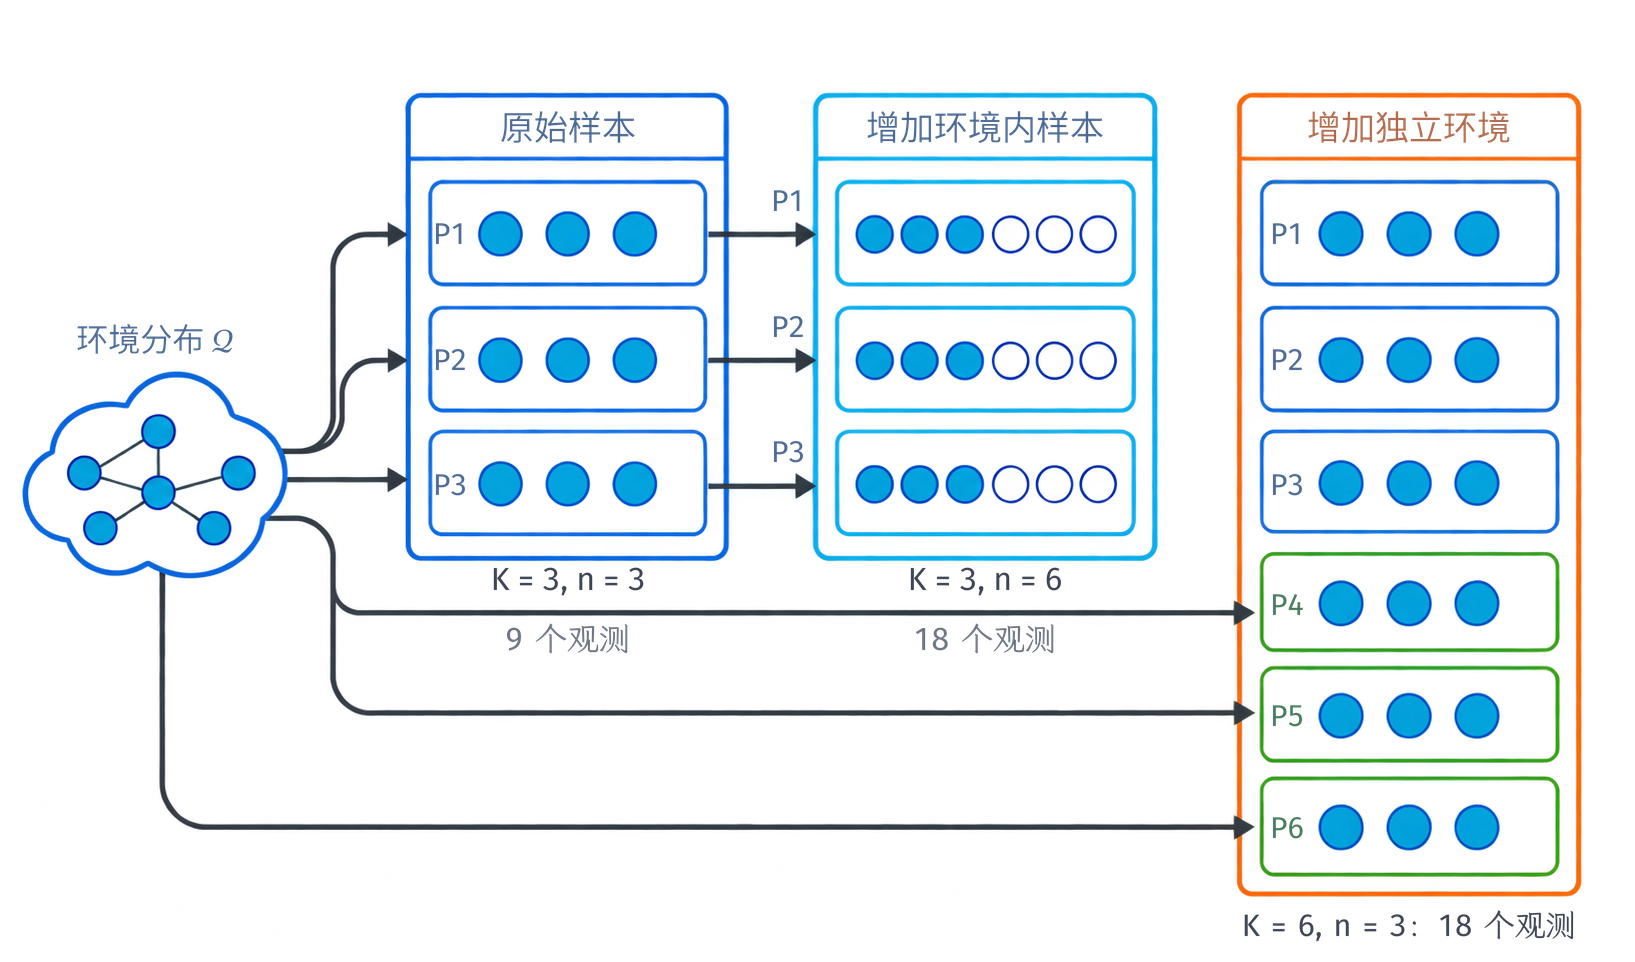
\includegraphics[width=164.600mm]{figures/03-foundations/02-learning-theory/generated/learning-theory-environment-sampling/figure.png}
  \caption{环境数量$K$与环境内样本数$n$对应不同的抽样层。每行边界代表一个环境，
 圆点代表其中的观测。左侧从同一环境分布$\mathcal Q$独立抽取3个环境，各取3个观测；
 中间的空心点表示在原有3个环境中继续抽取的观测，每个环境增至6个；右侧从$\mathcal Q$
 新抽取3个独立环境，每个环境仍取3个观测。
 中、右都有18个观测，只有右侧增加了独立环境数量。图中数量为教学构造，不对应实测数据。}
 \label{fig:learning-environment-sampling}
\end{figure*}
\FloatBarrier

记第$e$个环境的第$j$个观测为$z_{e,j}$，经验风险为
\[
 \widehat R(h)=\frac1{Kn}\sum_{e=1}^K\sum_{j=1}^n\ell(h,z_{e,j}).
\]
对包含$N$个候选、损失在$[0,1]$中的空间，把总体风险与经验风险之差拆成“环境抽样误差”和“给定环境后的观测误差”。分别使用Hoeffding不等式并对候选求和，以概率至少$1-\delta$得到
\begin{equation}
 \sup_h|R_{\mathcal Q}(h)-\widehat R(h)|
 \leq\sqrt{\frac{\log(4N/\delta)}{2K}}
     +\sqrt{\frac{\log(4N/\delta)}{2Kn}}.
 \label{eq:dg-two-level-uniform}
\end{equation}
第一项使用$K$个独立的环境风险，第二项在给定环境后使用$Kn$个独立但未必同分布的损失。ERM的环境平均超额风险不超过右侧的两倍，比较基准是$\inf_hR_{\mathcal Q}(h)$，始终只选同一个假设。增大域内$n$不能消除这个界中的有限环境代价；该结论也不能转换为对任意指定目标域的保证。

\Needspace{10\baselineskip}
\section{任务变化下的迁移可学习性}
\label{sec:task-transfer-learnability}

现在保持邮件的生成分布不变，只改变错误的计分方式。若仍能访问全部带标签邮件，我们可以直接按新损失重新训练。迁移问题更具体地问：只保留旧任务学到的知识，并提供有限的新任务反馈时，能否达到目标风险要求？要回答这一点，必须同时描述保留信息与目标学习过程。

\Needspace{7\baselineskip}
\subsection{学习问题}

\subsubsection{固定数据分布与变化的学习目标}

令一条完整观测为$z\in Z$，分布固定为$\mathcal P$，两个任务在共同候选空间$\mathcal H$上分别使用有界损失$\ell_S(h,z),\ell_T(h,z)\in[0,1]$。这里把损失写成假设与观测的函数，以容纳同一记录上的不同评价。相应风险为
\[
 R_S(h)=\mathbb E_{\mathcal P}\ell_S(h,z),\qquad
 R_T(h)=\mathbb E_{\mathcal P}\ell_T(h,z).
\]
本节下标$S,T$区分任务，分布始终是同一个$\mathcal P$；上一节中这两个下标区分域。改变损失可以改变最优决策，即使数据分布没有改变。

如果两个任务的输出形式不同，可以把$h$理解为包含所需输出的共同决策对象，再分别由损失读取相应部分。这个形式安排只提供统一记号，不会自动使两个任务相关。下面的推导直接采用同一输入、同一标签而错误代价不同的例子，避免把输出扩展本身当作迁移依据。

\subsubsection{可复用知识与目标任务的反馈}

源样本$S_S\sim\mathcal P^{n_S}$经过学习后产生知识$K=A_S(S_S)$，例如一个固定表示$\phi_K$。目标阶段只接收$K$和新的反馈样本$S_T$，由算法$A_T$输出$h$。样本中是否包含计算$\ell_T$所需的标签，属于反馈条件；只有输入时不能默认目标经验风险已经可算。

为使来源知识与新任务的估计误差能够分开，下面先令$S_T\sim\mathcal P^{n_T}$与$S_S$独立。条件于$K$以后，目标候选空间成为固定集合。若用同一批目标数据反复选择源模型、修改表示并估计最终风险，独立性就不再成立，需把这些选择纳入共同复杂度或使用新的验证数据。

\subsubsection{重新学习与知识迁移的比较基准}

设从原始输入重新学习时允许使用$\mathcal H$，复用$K$以后只使用非空候选子集$\mathcal H_K\subseteq\mathcal H$。例如，固定表示后只学习预测头，便限制了能够实现的输入到输出映射。用同一个总体、损失和大空间基准$R_{T,\mathcal H}^{\star}$比较，才能判断限制候选所节省的样本是否抵偿了表示损失。

如果只与$\inf_{h\in\mathcal H_K}R_T(h)$比较，一个始终输出错误常值的单元素空间也可能具有零超额风险。因此，迁移结论须同时报告受限空间的学习误差与相对于原空间的近似差。若来源阶段也消耗了大量样本，这些成本应与目标阶段的新增需求分别说明。

\Needspace{7\baselineskip}
\subsection{可学习的条件}

\subsubsection{源任务最优解的信息局限}

考虑只有一个输入、标签$y\in\{0,1\}$的教学例子。两种可能的固定数据分布分别满足$\mathbb P(y=1)=0.6$或$0.9$。源任务使用零一损失，两种情形的唯一最优分类器都输出1。因此，若来源知识只保存这个最优类别决策，目标阶段收到的信息完全相同。

现在把标签0预测为1的代价设为0.8，把标签1预测为0的代价设为0.2，正确预测代价为0。设正类概率为$p$，预测1与预测0的目标风险分别是$0.8(1-p)$和$0.2p$，故最优阈值为$p=0.8$。在$p=0.6$时应预测0，选错的超额风险为0.2；在$p=0.9$时应预测1，选错的超额风险为0.1。

仅接收源最优类别、没有新标签的目标算法无法区分这两种情形。若它以概率$q$输出1，则在第一种情形以概率$q$产生大于0.05的超额风险，在第二种情形以概率$1-q$失败，至少一个失败概率不小于$1/2$。每一种情形内部的数据分布都没有随任务改变；缺失的是源决策没有保留的概率信息。增加目标标签或保留概率估计会改变这一信息条件。

\subsubsection{共享表示对目标任务的充分性}

对固定表示$\phi_K$，目标阶段可用$g\circ\phi_K$预测，其中$g$属于允许的预测头集合。若表示把两个原始输入映射到同一点，任何预测头都必须对它们作出相同决策。在只含这两个输入的例子中，若它们都以正概率出现，且各自的目标最优决策唯一而不同、原始候选能够同时实现这两个决策，那么合并它们就会产生目标近似误差。源任务不需要区分它们，也不能消除这个目标任务的损失。

为了量化这一影响，定义
\begin{equation}
 a_T(K)=\inf_{h\in\mathcal H_K}R_T(h)
        -\inf_{h\in\mathcal H}R_T(h)\geq0.
 \label{eq:task-transfer-bias}
\end{equation}
$a_T(K)=0$表示受限空间能够任意逼近大空间的目标最优风险，不要求最小值一定取到。表示对目标预测足够使用，还取决于预测头是否能够表达所需决策。源任务风险小并不能单独限制$a_T(K)$；要给出端到端保证，需由任务联系或源学习分析进一步控制这个量。

\subsubsection{源任务风险与目标任务风险的联系}

记源任务的类内最优风险为$R_{S,\mathcal H}^{\star}=\inf_{h\in\mathcal H}R_S(h)$。一种直接的充分条件，是存在已知的候选转换$T:\mathcal H\to\mathcal H$和统一常数$c\geq0,b\geq0$，使允许的分布与任务对都满足
\begin{equation}
 R_T(T(h))-R_{T,\mathcal H}^{\star}
 \leq c\bigl(R_S(h)-R_{S,\mathcal H}^{\star}\bigr)+b.
 \label{eq:task-risk-transfer}
\end{equation}
它说明源任务的近似最优解经转换后，离目标最优还有多远。若源算法以高概率保证超额风险至多$\varepsilon_S$，则转换所得目标超额风险至多$c\varepsilon_S+b$。只有$b$可消除或被进一步学习控制时，这条路线才能支持任意精度的目标PAC要求。

这个条件需要证明，不能由“两个任务相关”替代。例如若$\ell_T(h,z)=c\ell_S(h,z)+d(z)$，其中$c>0$且$d$与$h$无关、相应风险有限，则取$T$为恒等映射即可得到$b=0$，因为与决策无关的期望项在超额风险中抵消。前面的代价变化反例则表明，一般的损失改变未必具有这种性质。

如果源任务保留的是概率信息，而不是一个最优类别，改变错误代价仍可能得到保证。为说明这一点，回到二分类，但在这个例子中让源任务用平方损失学习条件正类概率$\eta(x)=\mathbb P(y=1\mid x)$，输出$f(x)\in[0,1]$。这里比较的是全部可测预测器中的Bayes最优风险，而不是前面固定$\mathcal H$中的最优风险。对平方损失按输入取条件期望，交叉项因$\mathbb E[y-\eta(x)\mid x]=0$而消失，得到
\[
 R_S(f)-R_S(\eta)=\mathbb E[(f(x)-\eta(x))^2].
\]
因此，源超额风险控制了保留概率的均方误差。

设目标任务把标签0预测为1的代价设为$c_0\in(0,1]$，把标签1预测为0的代价设为$c_1\in(0,1]$，正确预测不受罚。给定$x$，两个决策的条件风险分别为$c_0(1-\eta(x))$和$c_1\eta(x)$，故目标阈值为$\tau=c_0/(c_0+c_1)$。用源概率构造$d_f(x)=\mathbb I\{f(x)\geq\tau\}$，对应Bayes决策为$d_\eta$。只有二者决策不同才产生超额风险；这时$\tau$位于$f(x)$与$\eta(x)$之间，故$|\eta(x)-\tau|\leq|f(x)-\eta(x)|$。于是
\begin{align*}
 R_T(d_f)-R_T(d_\eta)
 &= (c_0+c_1)\mathbb E\bigl[|\eta(x)-\tau|
       \mathbb I\{d_f(x)\neq d_\eta(x)\}\bigr] \\
 &\leq(c_0+c_1)\mathbb E|f(x)-\eta(x)| \\
 &\leq(c_0+c_1)\sqrt{R_S(f)-R_S(\eta)}.
\end{align*}
最后一步使用Cauchy--Schwarz不等式。若源概率学习具有相对于$\eta$的高概率保证，这个界便将它转为新代价下的保证，无需再估计目标标签分布。与仅保存类别的反例相比，新增依据是概率估计保留了移动阈值需要的信息；若源候选不能逼近$\eta$，相应近似差仍须计入。


\Needspace{7\baselineskip}
\subsection{有限样本保证}

\subsubsection{源知识估计误差与目标任务学习误差}

有目标标签时，我们可以在$\mathcal H_K$中重新选择决策。目标超额风险自然分成两部分：在这个空间内没有学到最优的误差，以及空间本身相对于$\mathcal H$的近似差$a_T(K)$。如果来源阶段以概率至少$1-\delta_S$保证$a_T(K)\leq b_S$，目标阶段再给出条件失败概率$\delta_T$的学习保证，两类失败合计至多$\delta_S+\delta_T$。

这里的$b_S$必须来自明确的源学习结果与任务联系，不能把源经验误差直接改名为$b_S$。下一结论先条件于实际得到的$K$，说明目标阶段可以做到什么；它将来源知识的好坏保留为显式项。

\subsubsection{固定表示下的目标任务样本复杂度}

为看清样本量的作用，设每个可能的$K$都确定一个有限非空空间$\mathcal H_K$，且$|\mathcal H_K|\leq N_0$。这些候选可以是固定表示配合一组允许的预测头。目标算法计算每个候选的新损失平均值，再选择近似最小者。

\begin{theorem}[复用知识后的目标风险保证]
\label{thm:task-transfer-finite}
设$K$与目标样本$S_T\sim\mathcal P^n$独立，$\mathcal H_K\subseteq\mathcal H$满足上述大小限制，目标损失可测且属于$[0,1]$。若输出$\widehat h\in\mathcal H_K$的目标经验风险至多比类内最小值高$\rho$，则以概率至少$1-\delta$，
\begin{equation}
 R_T(\widehat h)-R_{T,\mathcal H}^{\star}
 \leq a_T(K)+\sqrt{\frac{2\log(2N_0/\delta)}{n}}+\rho.
 \label{eq:task-transfer-finite}
\end{equation}
\end{theorem}
\begin{proof}
条件于$K$，候选空间固定，目标样本仍独立同分布。对候选损失使用Hoeffding不等式并求和，得到统一偏差上界
\[
 \sqrt{\frac{\log(2N_0/\delta)}{2n}}.
\]
近似ERM使用两次偏差与一次优化误差，因而在类内达到根号项加$\rho$的超额风险。再加入式~\eqref{eq:task-transfer-bias}即得结论。该条件概率保证对每个$K$成立，对$K$平均后仍成立。
\end{proof}

若$a_T(K)=0$且$\rho=0$，则$n\geq2\log(2N_0/\delta)/\varepsilon^2$足够。这给出一种统计可行的目标学习规则；要成为可执行程序，还需候选损失可计算且比较可实现。若预测头空间无限，可以用目标损失族的Rademacher复杂度等量替换有限候选的对数项；固定表示只限制候选结构，并不自动保证复杂度小或优化容易。

\subsubsection{迁移降低样本需求的条件}

假设直接学习的有限空间大小为$N$，复用后为$N_0<N$，二者的损失和评价总体一致。上述充分界把目标抽样代价中的$\log N$换成$\log N_0$；这个改善需要$a_T(K)$与优化误差不抵消所节省的估计误差。因此，更小的受限空间只是减少目标样本需求的一条条件性途径，不是任意压缩都有效的结论，也不能由两个上界直接推出最优样本复杂度的严格排序。

多任务表示理论进一步研究哪些来源任务足以确定对目标有用的表示。代表性结果把共享表示、任务专属预测头及来源任务的多样性分别纳入分析，在相应任务联系下得到目标样本需求的改善\scite{tripuraneni2020diversity}。这类研究需要明确任务族；把任意新损失都纳入目标集合，会使表示充分性要求明显增强。

\subsubsection{任务联系不足时的迁移边界}

若$a_T(K)>0$固定不变，再多目标样本也只能让算法接近受限空间的最好结果。允许重新学习表示会扩大候选空间，可能降低近似差，同时增加估计和计算代价。若完全没有目标反馈，又不存在式~\eqref{eq:task-risk-transfer}这样的联系，源任务成功本身不能排除前面的不可识别反例。

负迁移应在相同目标样本、评价分布和可比训练预算下，与直接学习基准比较；它表示复用旧知识使目标风险变大。理论分析需要确定增加的是近似误差、估计误差还是优化误差。一个宽松的风险上界变大，并不足以证明实际发生了负迁移。

\section{持续学习的可学习性}
\label{sec:continual-learnability}

继续按月份接收邮件，并要求模型能处理已经出现过的邮件类型。当前数据可以让模型更适合本月，却可能使过去的决策失效。本节先明确历史评价，再给出保留损失统计量的有限候选算法，说明不重访原始数据时仍可能学习；同时用记忆下界说明，历史信息也不能任意丢弃。

\Needspace{7\baselineskip}
\subsection{学习问题}

\subsubsection{固定任务与持续到达的数据}

固定可测空间$Z=X\times Y$、假设空间$\mathcal H$和损失$\ell\in[0,1]$。第$t$阶段接收$S_t=(z_{t,1},\ldots,z_{t,n_t})$，其中$z_{t,i}$来自$\mathcal P_t$。下面的有限样本结论先固定分布序列，并假定各阶段内独立同分布、不同阶段样本相互独立。序列可以变化，但不依赖已经抽取的训练样本；由历史自适应选择分布的过程需要另外的条件概率分析。

为描述旧数据离开后算法还能使用什么，令$M^{(t)}$表示第$t$阶段结束时的全部保留状态，并写成
\[
 M^{(t)}=U_t(M^{(t-1)},S_t),\qquad
 h^{(t)}=V_t(M^{(t)}).
\]
$U_t$为更新规则，$V_t$为预测规则，带括号的上标表示阶段。本节评价每次更新完成后，模型在各分布中新观测上的期望损失，不评价反馈到达前的在线预测损失。状态包括模型参数和所有历史摘要；除这个状态之外，算法不能再读取已经离开的样本。

\subsubsection{分布变化与历史数据的不可重访}

若只在当前$S_t$上最小化损失，算法估计的是$\mathcal P_t$下的风险。要维持历史表现，需要让状态保留与历史评价相关的信息。保存若干旧样本是一种方式，保存可直接更新的损失统计量是另一种方式；它们支持的候选空间与计算要求并不相同。

没有重访原始数据，不排除保留足以计算既定经验目标的统计量；有限维状态也不必然意味着有限比特。因此，以下正面构造明确保存哪些计数，反例则把包括最终模型在内的全部历史状态限制为$B$比特。这样可以比较信息的需求，而不会把未计入的参数存储当作免费记忆。

\subsubsection{当前风险、历史风险与遗忘}

对每个历史阶段$i$，定义$R_i(h)=\mathbb E_{\mathcal P_i}\ell(h,z)$和$R_i^\star=\inf_{h\in\mathcal H}R_i(h)$。为了让每个已经出现的阶段在评价中占同样权重，取
\begin{equation}
 \overline R_t(h)=\frac1t\sum_{i=1}^tR_i(h).
 \label{eq:continual-average-risk}
\end{equation}
它比较同一个模型在历史分布上的平均表现；若实际使用频率不同，应在观察样本之前规定相应权重。平均评价的类内基准是$\inf_h\overline R_t(h)$，不能把它换成允许每个阶段各选模型的$t^{-1}\sum_iR_i^\star$。

对已经学过的阶段$i$，$R_i(h^{(t)})-R_i(h^{(i)})$度量之后更新造成的风险变化，正值表示遗忘。但遗忘小也可能只是一直表现很差，所以还需看$R_i(h^{(t)})-R_i^\star$。如果要求所有历史分布都接近各自最优，就应控制$\max_{i\leq t}[R_i(h^{(t)})-R_i^\star]$。最大值在此用于防止少数历史环境被平均掩盖。

对给定允许序列族和记忆预算，平均风险的有限阶段PAC要求可表述为：对任意$\varepsilon,\delta\in(0,1)$和预定阶段数$T$，存在统一的有限样本门槛与遵守预算的同一算法，对允许族内的每个分布序列，都以概率至少$1-\delta$保证全部$t\leq T$的平均超额风险不超过$\varepsilon$。逐历史分布要求则把这个风险量换成最大逐域超额风险。有限$T$下可学习并不自动意味着同一固定预算能够支持无限阶段。

\Needspace{7\baselineskip}
\subsection{可学习的条件}

\subsubsection{不同历史分布上的预测兼容性}

如果两个历史环境都只产生同一个输入，一个总标为0，另一个总标为1，那么任何固定二分类器至少在一个环境上风险为1。两个环境分别都可零风险学习，但不提供环境身份的同一个分类器无法同时实现这一目标。即使全部数据都保留，这个表达限制也不会消失。

为了把这种限制与抽样误差分开，定义共同候选能达到的最小最大超额风险
\begin{equation}
 \Delta_t=\inf_{h\in\mathcal H}\max_{i\leq t}[R_i(h)-R_i^\star].
 \label{eq:continual-compatibility}
\end{equation}
内部最大值反映需要保持的每个历史分布，外部下确界在允许的共同模型中选择最好者。有限空间中$\Delta_t=0$意味着存在同时最优的候选；$\Delta_t>0$时，任意共同模型的最大逐域超额风险都至少为$\Delta_t$。平均风险相对于共同模型最优者的学习要求，仍可能成立。

\subsubsection{保持历史表现所需的信息}

固定$N$个候选，如果学习目标只是所有观测的平均损失，就可以在数据离开前为每个候选累加损失。原始邮件随后丢弃，累计值仍能用于选择经验最优者。这说明能否保持历史表现，取决于状态是否保留当前学习目标所需的信息，而不只取决于是否保存原始样本。

这个构造依赖候选在观测到来前已经固定。若以后增加了一个新模型，它在旧样本上的损失通常无法由原有候选的累计值恢复。对不断改变表示的神经网络，也不能直接把有限候选计数法理解为一个固定大小的通用摘要。

\subsubsection{稳定性与可塑性的共同要求}

如果状态只允许输出初始模型，历史能力可以保持不变，但新分布上的超额风险可能始终很大。如果状态只保留最新批次的最优模型，又可能丢失旧环境的决策。有效的学习过程需要在既定评价目标下同时约束这两方面，而不是分别把“参数不变”或“当前误差下降”当作成功。

理论上，这些约束体现为候选是否兼容、历史目标能否估计以及更新是否足够接近经验最优。记忆下界描述信息必须保留多少，优化分析描述保留这些信息以后算法能否利用它们。二者都需要与总体风险保证结合。

\subsubsection{信息丢失与有限记忆下的不可能性}

下面用固定分类任务说明存储要求。令$X=\{1,\ldots,T\}$，每个输入$i$有一个固定但未知的标签$b_i\in\{0,1\}$。第$i$阶段的分布集中在$(i,b_i)$，学习器完整看到该标签，之后旧观测不可重访。所有二分类函数都允许，因而存在一个共同的零风险模型；困难只在保留任意标签串所需的信息。

\begin{theorem}[逐历史分布保持的信息下界]
\label{thm:continual-memory-example}
在上述设定中，取正整数$T$及$\delta\in(0,1)$，假定最终预测函数只能由至多$B$比特的保留状态和与数据独立的随机性产生，全部历史相关存储均计入状态。若要求对每个标签串，以概率至少$1-\delta$输出一个在所有$T$个历史分布上风险均小于1的确定性二分类函数，则
\[
 B\geq T+\log_2(1-\delta).
\]
概率针对学习与模型选择的随机性，输出后对每个输入使用所选函数。
\end{theorem}
\begin{proof}
每个历史分布集中于一个点，风险小于1意味着该点预测正确。因此成功等价于恢复完整标签串。先固定所有独立随机数；至多$2^B$种状态只能解码为至多$2^B$种函数，故在$2^T$个等概率标签串中，成功比例不超过$2^{B-T}$。再对随机数平均，上界不变。若对每个标签串的成功概率都至少为$1-\delta$，平均成功概率也至少为该值，所以$1-\delta\leq2^{B-T}$。
\end{proof}

这个教学反例中，每阶段标签已经完全揭示，增加该阶段重复样本不能减少记忆需求。它说明任意扩大的独立历史信息与固定比特预算不能同时满足任意序列上的逐域保持。它不排除具有共享结构、较弱平均目标或可重访条件的正面结果；一般PAC持续学习中的存储与访问次数关系还可参考相应复杂度研究\scite{chen2022memory}。

\Needspace{7\baselineskip}
\subsection{有限样本保证}

\subsubsection{历史分布上的平均风险保证}

先考虑有限非空空间$\mathcal H$，大小为$N$，并在每个阶段接收$n$个独立样本。候选事先固定，算法为每个$h$维护累计损失
\[
 C_t(h)=C_{t-1}(h)+\sum_{j=1}^n\ell(h,z_{t,j}),\qquad C_0(h)=0.
\]
在第$t$阶段结束时，选择累计损失最小的候选，即最小化$\widehat R_t(h)=C_t(h)/(tn)$。因为各阶段样本数相同，这个经验量估计式~\eqref{eq:continual-average-risk}规定的等权历史风险。

\begin{theorem}[累计损失学习的历史平均保证]
\label{thm:continual-average-finite}
在固定分布序列、阶段内及阶段间独立抽样、有界损失和有限候选的上述条件下，预先给定$T\geq1$。若每阶段输出的经验风险至多比最小值高$\rho_t$，则以概率至少$1-\delta$，所有$t\leq T$同时满足
\begin{equation}
 \overline R_t(h^{(t)})-\min_{h\in\mathcal H}\overline R_t(h)
 \leq\sqrt{\frac{2\log(2NT/\delta)}{tn}}+\rho_t.
 \label{eq:continual-average-bound}
\end{equation}
\end{theorem}
\begin{proof}
对固定$t,h$，$tn$个损失相互独立、属于$[0,1]$，虽然不一定同分布，其平均期望仍为$\overline R_t(h)$。Hoeffding不等式给出
\[
 \mathbb P\{|\widehat R_t(h)-\overline R_t(h)|>a\}
 \leq2\exp(-2tn a^2).
\]
对$N$个候选和$T$个阶段求和，以总失败概率$\delta$控制每阶段偏差
$a_t=\sqrt{\log(2NT/\delta)/(2tn)}$。各阶段经验最优性再给出$2a_t+\rho_t$的超额风险界。
\end{proof}

若精确最小化，令$n\geq2\log(2NT/\delta)/\varepsilon^2$便保证全部$t\leq T$达到精度$\varepsilon$，这是包含最早阶段要求的充分条件。当候选和损失可计算且候选间的比较可实现时，算法每条观测评估$N$个候选并更新计数，展示了不保留原始样本的一条可行路径；当$N$巨大时，计算代价仍可能难以接受。

对零一损失，每个计数属于$\{0,\ldots,Tn\}$，除固定候选描述外，保存累计值需要至多$N\lceil\log_2(Tn+1)\rceil$比特。一般实值损失需另外规定量化精度；若每次量化绝对误差至多为$q$，平均损失误差也至多为$q$，上述超额风险界再增加$2q$。因此不能把$N$个实数计数直接说成与精度无关的有限比特保证。

\subsubsection{各历史分布上的同时风险保证}

平均风险小并不保证每个历史分布的风险都小。例如，等权的$T$个环境中，一个环境风险为1、其余为0，平均风险只有$1/T$。若每个环境都必须保持，就需要保存能够分别估计其风险的信息。对有限候选，可以保留每个阶段、每个候选的经验风险$\widehat R_i(h)$。

为了比较各环境相对于自身最好候选的差距，定义
\[
 \widehat E_t(h)=\max_{i\leq t}
 \left[\widehat R_i(h)-\min_{g\in\mathcal H}\widehat R_i(g)\right].
\]
算法选择使$\widehat E_t$近似最小的候选。减去各自经验最优值，是为了避免把不同环境固有的噪声差异直接解释为遗忘；最大值则落实每个历史环境都要保持的要求。

\begin{theorem}[有限候选的逐历史分布保证]
\label{thm:continual-uniform-finite}
沿用上一结论的抽样、损失和有限候选条件。令
$a=\sqrt{\log(2NT/\delta)/(2n)}$。若每阶段输出满足
$\widehat E_t(h^{(t)})\leq\min_h\widehat E_t(h)+\rho_t$，则以概率至少$1-\delta$，所有$t\leq T$同时满足
\begin{equation}
 \max_{i\leq t}[R_i(h^{(t)})-R_i^\star]
 \leq\Delta_t+4a+\rho_t.
 \label{eq:continual-uniform-bound}
\end{equation}
\end{theorem}
\begin{proof}
对全部阶段与候选求和，Hoeffding不等式保证同一事件上
$|\widehat R_i(h)-R_i(h)|\leq a$。于是经验最优值与总体最优值的差也至多为$a$，每个候选的经验超额风险与真实超额风险之差至多为$2a$。取最大值保持这一误差界；再比较经验近似最小者与真实最小者，两次使用$2a$并加入$\rho_t$，即得结论。该事件已覆盖所有$i\leq T$，故结论同时覆盖每个前缀$t$。
\end{proof}

若所有历史分布存在共同最优候选，则$\Delta_t=0$。精确求解时，$n\geq8\log(2NT/\delta)/\varepsilon^2$足以给出每阶段、每历史分布的精度$\varepsilon$。若$\Delta_t>0$，结论只保证接近共同模型能达到的最好折中，不能称为相对于每个独立最优基准的任意精度PAC学习。

\subsubsection{样本数量、记忆容量与序列长度}

两条正面结果保存的信息不同。累计损失足以选择历史平均风险小的候选，计数数量为$N$；分别保持历史环境需要上述构造保存$Nt$个阶段计数。后者是一种充分实现方式，不是所有算法都必须使用的存储下界。共同结构或更合适的摘要可能减少存储，但需要另外证明摘要仍支持所要求的风险控制。

两条界的样本依赖也不同。平均评价利用$tn$个观测，而逐域估计中每个环境仍只有$n$个样本；不断增加新环境的数据，并不自动提高早期环境风险的估计精度。有限阶段上的$\log T$来自同时控制失败事件。若要求无限阶段同时成立，可以为第$t$阶段分配可求和的失败预算，如$6\delta/(\pi^2t^2)$；但这样只处理概率累计，并不消除不断增长的存储或兼容性要求。

这些结果允许不同阶段分布不同，但依赖固定序列与独立抽样。存在时间相关、模型反馈影响数据分布或任务边界未知时，需要先重建抽样模型，再判断哪些集中不等式与统计摘要仍然适用。阶段数本身不能概括这些依赖。

\subsubsection{多次更新中的误差累积与控制}

如果具体算法没有重新求解历史经验目标，而只对上一步模型做局部更新，就需要控制每次更新给旧分布带来的风险增量。假设第$j$次更新在所有$i<j$上都满足
$R_i(h^{(j)})-R_i(h^{(j-1)})\leq\gamma_j$，则对任意$i<t$，逐项相加得到
\[
 R_i(h^{(t)})-R_i(h^{(i)})\leq\sum_{j=i+1}^t\gamma_j.
\]
即使每一步的增量都很小，不可求和的增量仍可能累积。若各步保证带有失败概率，也需要对对应事件作联合控制。

风险增量条件必须有历史信息或结构假设支持，不能仅由当前训练误差下降推出。有限候选下，若保存的历史样本对所有候选同时给出误差$a_i$的风险估计，那么两次模型在该环境上的真实风险差，至多比经验风险差大$2a_i$。统一控制候选使样本可以用于数据依赖的模型比较；只有对一个预先固定模型成立的估计，不能直接用于反复选出的新模型。

累计损失与逐域经验超额风险构造直接控制每个阶段的总体目标，不需要把每次遗忘上界累加。对参数化模型，任务顺序、更新方向与参数约束如何改变遗忘及泛化，则需结合具体模型分析。线性模型下已有研究分别刻画这些因素，不能把其条件下的结论直接推广为任意神经网络的保证\scite{lin2023forgetting}。

\section{本章小结}
\label{sec:transfer-learning-summary}

同样是把已有经验用于后续预测，三种设定的信息要求不同。分布变化时，需要连接源观测与目标标签规律；目标任务变化时，需要确认旧知识保留了新损失所需的信息；持续学习时，还要保证历史信息在更新过程中没有丢失到无法支持评价的程度。只有明确这些联系，有限样本工具才能把经验结果变成总体保证。

分布迁移中的重加权说明，跨域条件可以把目标风险写成可估计的源期望；任务迁移中的受限空间分析则把表示近似差与目标学习误差分开。两者都要求控制优化误差，且当前上界中的固定残余不能通过单纯增加样本消除；这并不自动构成不可学习的下界。存在一个正确候选也不够：相同可见信息若要求冲突决策，学习仍会失败。

持续学习的正面构造说明，原始数据不可重访并不必然阻止学习，适合评价目标的统计量有时已经足够。但历史平均保证、逐历史分布保证和遗忘控制具有不同的比较基准与资源要求。共同模型的兼容性限定可以达到的风险，有限状态限定能够保留的信息，样本与计算资源决定这些目标能否实现；逐阶段的成功还需明确扩展到多长的序列。

\paragraph{扩展阅读}
Ben-David等人的领域自适应分析把源风险、输入分歧与共同错误联系起来；其不可学习性研究适合与本章反例对照，检查哪些可观察相似性仍不足以支持目标保证\scite{bendavid2010adaptation,bendavid2010impossibility}。

Tripuraneni、Jordan与Jin研究来源任务的多样性如何支持共享表示及新任务的样本效率。Maurer、Pontil与Romera-Paredes则从多任务表示学习分析共享结构的收益。阅读时应分别核对任务抽样、表示假设和新任务反馈，不能把这些结果理解为对任意任务变化的统一承诺\scite{tripuraneni2020diversity,maurer2016representation}。

Chen、Papadimitriou与Peng从PAC框架研究持续学习的记忆需求及多次访问任务带来的改变，可用于比较一次读取、重访与状态容量的关系。Lin等人在线性模型下分析遗忘与泛化，适合进一步理解任务联系、参数规模和顺序为何需要同时进入理论条件\scite{chen2022memory,lin2023forgetting}。
